% Current implemented method. This section does not describe the historical
% sparse-JL proposal in the received abstract and introduction.
\section{Methodology}
\label{sec:methodology}
The purpose of the audit is to determine whether a proposed prototype bank
reduces the nearest-center cost on a committed feature catalog. Repeating an
exact distance proof for every candidate incurs work in the original feature
dimension. We instead authenticate the deployed model's groups once, compute
their assigned-center cost change exactly, and bound the additional change
caused by records switching groups. The resulting interval supports a strict
decision, with authenticated row corrections and exact fallback for ambiguous
updates.

\subsection{Problem Formulation}
\label{sec:methodology-problem}
Let $X=(x_1,\ldots,x_n)$, $x_i\in\mathbb Z^d$, denote the owner's quantized
feature catalog, and let $C^0=(c^0_0,\ldots,c^0_{k-1})$ be the deployed
prototype bank. The owner commits to the ordered catalog, the quantizer and
the deployed model. Given an approved candidate $C^1$ with the same number
and indexing of centers, define
\begin{equation}
 \begin{aligned}
 \Phi_X(C)&=\sum_{i=1}^{n}\min_{0\leq j<k}\|x_i-c_j\|_2^2,\\
 \Delta&=\Phi_X(C^1)-\Phi_X(C^0).
 \end{aligned}
 \label{eq:methodology-objective}
\end{equation}
The required output is an authenticated interval $[L,U]$ containing a
positive integer multiple of $\Delta$. An upper endpoint below zero
certifies improvement; a lower endpoint above zero certifies worsening.
The interval $[0,0]$ certifies equality. Other intervals containing zero
require further computation.

One audit episode fixes $X$ and $C^0$ while comparing several candidates,
such as prototype updates obtained from new training minibatches at different
update rates. Every center may change, and candidate values may arrive after
preprocessing. Installing a new deployed bank starts a new episode and
requires new group preprocessing. The statement concerns the complete
committed catalog and the quantized objective in
Eq.~\eqref{eq:methodology-objective}. The feature extractor and its training
are supplied by the owner rather than certified by the audit.

\subsection{Reusable Prototype-Update Certificates}
\label{sec:methodology-pipeline}
The method has four stages. First, a frozen basis defines compact features
and residual energies. Second, preprocessing authenticates those statistics,
the exact deployed assignments and their group moments. Third, a candidate
query combines an exact group-level change with bounded switching terms.
Fourth, exact checks on a small set of rows tighten an inconclusive interval
before complete exact fallback. Figure~\ref{fig:methodology-pipeline}
summarizes the computations shared across candidates and those repeated for
each update.
\begin{figure*}[tbp]
\centering
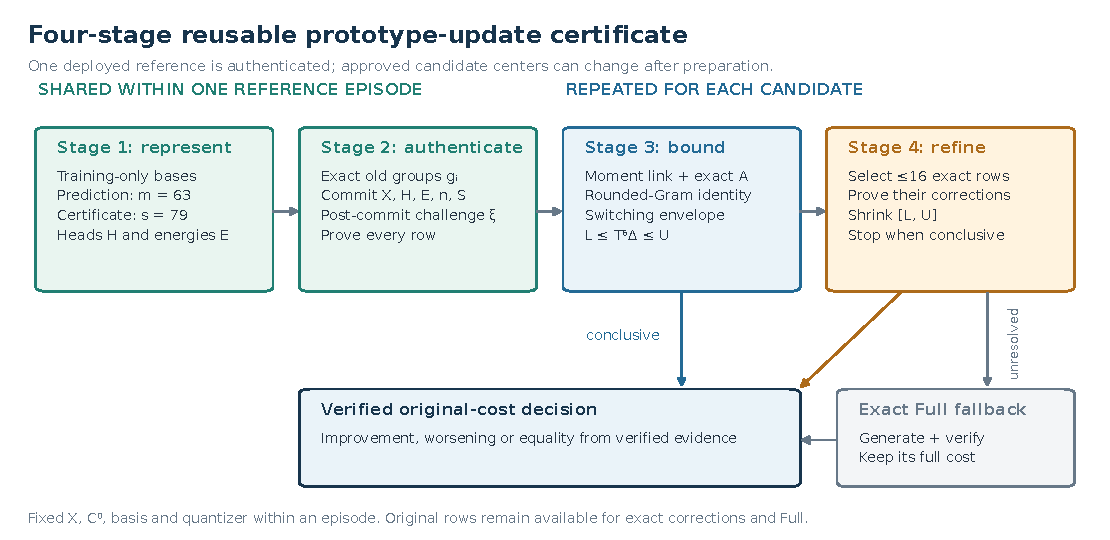
\includegraphics[width=.96\textwidth]{paper_results/ccd_pilot_20261029/figures/methodology_four_stages.pdf}
\caption{The four-stage prototype-update certificate. Stages 1--2 prepare
the compact representation and authenticate exact old memberships and row
statistics for one reference episode. Stage 3 proves moment linkage and the
exact assigned contribution, then bounds switching for each approved new
bank. Stage 4 proves selected exact corrections or invokes proved Full
fallback. The original rows remain available to the prover.}
\label{fig:methodology-pipeline}
\end{figure*}


\subsubsection{Stage 1: Compact Representation and Residual Energy}
\label{sec:methodology-representation}
The representation uses a public integer basis $B\in\mathbb Z^{s\times d}$,
a positive scale $T$ and the anchor $a=c^0_0$. For any feature vector or
center $v$, define
\begin{align}
 H_B(v)&=TB(v-a),\nonumber\\
 R_B(v)&=(T^2I_d-B^\top B)(v-a),\nonumber\\
 E_B(v)&=\|R_B(v)\|_2^2.
 \label{eq:methodology-statistics}
\end{align}
These integer statistics retain the projected coordinates and a bound on
the discarded directions. We write $H_i=H_B(x_i)$ and $E_i=E_B(x_i)$ for
stored row values. Projection with residual information is an
established clustering-summary construction
\cite{feldman2013tiny,feldman2020tiny}. Here it supplies the inputs to a
verified cost-change certificate.

\paragraph{Basis construction}
The centroid-informed basis begins with an orthonormal basis for
$\operatorname{span}\{c^0_j-c^0_0:j>0\}$. Training rows are translated by
$a$, projected away from this span and mean-centered. PCA directions of
these training residuals complete the prediction basis. Reprojection and
orthonormalization remove overlap before its coefficients are rounded at
scale $T$. The PCA baseline instead obtains its entire prediction basis
from the same training rows. Neither construction uses held-out catalog
rows or future candidate centers to fit its directions.

The implemented profile fixes a prediction rank $m=63$ and appends 16
training-residual SVD directions for a certificate rank $s=79$, using
$T=2^{14}$. The first $m$ rounded rows remain unchanged. The certificate
statistics are authenticated for the wider basis independently of the
prediction model. These values define the evaluated profile; the mechanism
also applies to other admitted ranks and scales.

\paragraph{Prediction and assignment certificates}
Using the prediction basis $B_m$, the approximate assignment is
\begin{equation}
 \widehat g_i(C)=\mathop{\arg\min}_{j}
 \left[\|H_{B_m}(x_i)-H_{B_m}(c_j)\|_2^2
       +E_{B_m}(c_j)\right],
 \label{eq:methodology-prediction}
\end{equation}
with lowest-index tie breaking. The omitted term $E_{B_m}(x_i)$ is common
to all centers. Assignment agreement with exact Full, the fraction of
individually certified assignments, and the fraction of certified update
decisions measure different outputs. Section~\ref{sec:methodology-switching}
gives pairwise bounds that can certify a predicted label; the wider basis
is used for the aggregate cost-change decision without changing
Eq.~\eqref{eq:methodology-prediction}. Assignment metrics are evaluated by
the native reference. The implemented group verifier returns aggregate
cost-change intervals rather than individual labels or certificate flags.
All bounds are deterministic for the
fixed rounded basis. The selected profile uses no JL projection or random
projection tail.

\subsubsection{Stage 2: Authenticated Groups and Exact Group Moments}
\label{sec:methodology-groups}
For each record, let
\begin{equation}
 \begin{aligned}
 g_i&\in\mathop{\arg\min}_{0\leq j<k}\|x_i-c^0_j\|_2^2,\\
 n_g&=\sum_i\mathbf1[g_i=g],\qquad S_g=\sum_{i:g_i=g}x_i.
 \end{aligned}
 \label{eq:methodology-groups}
\end{equation}
Any minimizing deployed group is valid; the native builder uses the first
minimizer. Exact membership follows by comparing the linear scores
$\|c^0_j\|_2^2-2\langle x_i,c^0_j\rangle$, since $\|x_i\|_2^2$ is common.
Preprocessing proves this membership rather than trusting a native label.

\paragraph{Binding rows, derived values and moments}
Salted Poseidon2 Merkle commitments bind the ordered original rows and the
derived leaves $(H_B(x_i),E_B(x_i),g_i)$, together with their model context
\cite{poseidon22023}. A separate salted commitment binds all $n_g,S_g$ to
the same roots and model. Each row proof checks same-index openings,
Eq.~\eqref{eq:methodology-statistics}, coordinate ranges and exact deployed
membership. The verifier requires every catalog index exactly once.

The moments are linked to the complete row collection with a polynomial
fingerprint. After the original, derived and moment commitments are fixed,
an independent auditor issues a nonzero uniform challenge
$\xi\in\mathbb F_p^*$. For coordinate indices $t=0,\ldots,d-1$, set
\begin{align}
 P_i(\xi)&=1+\sum_{t=0}^{d-1}x_{it}\xi^{t+1},\nonumber\\
 z_{ig}&=\mathbf1[g_i=g]P_i(\xi)+\mu_{i+1,g}-\mu_{ig},
 \label{eq:methodology-fingerprint}
\end{align}
where the $\mu_{ig}$ are private field masks. Row proofs bind adjacent mask
vectors through indexed hashes. Complete coverage and adjacent-hash equality
make the internal masks telescope. A moment-link relation checks
\begin{equation}
 \sum_i z_{ig}=n_g+\sum_{t=0}^{d-1}S_{gt}\xi^{t+1}
                    +\mu_{n+1,g}-\mu_{1g}\pmod p.
 \label{eq:methodology-moment-link}
\end{equation}
Counts and coordinate sums have explicit integer ranges. The owner retains
the model, roots, challenge receipt and approved verification-key hashes
independently of the prover's bundle.

\paragraph{Exact assigned-center change}
For a new approved bank, the linked group statistics give
\begin{equation}
 \mathcal A=
 \sum_{g=0}^{k-1}\left[
 2\langle S_g,c^0_g-c^1_g\rangle
 +n_g(\|c^1_g\|_2^2-\|c^0_g\|_2^2)\right].
 \label{eq:methodology-assigned}
\end{equation}
This is the exact change if every record keeps its deployed group. A
query proof combines the moment-link check with this expression, using the
approved original-space centers as public inputs. The remaining correction
for row $i$ is
\begin{equation}
 b_i=\min_j\|x_i-c^1_j\|_2^2-\|x_i-c^1_{g_i}\|_2^2\leq0,
 \qquad \Delta=\mathcal A+\sum_i b_i.
 \label{eq:methodology-decomposition}
\end{equation}
Thus the original-dimension group contribution is exact, and only switching
requires an uncertainty interval. In particular, an authenticated
$\mathcal A<0$ already suffices for improvement; the switching certificate
also addresses updates that this one-sided test leaves open.

\subsubsection{Stage 3: Integer-Safe Switching Bounds}
\label{sec:methodology-switching}
Rounding makes the rows of $B$ only approximately orthonormal. We retain the
resulting Gram correction instead of assuming $BB^\top=T^2I_s$. Let
\begin{equation}
 \begin{aligned}
 G&=BB^\top-T^2I_s,\\
 \mathcal D_B(x,c)&=\|H_B(x)-H_B(c)\|_2^2+E_B(x)+E_B(c).
 \end{aligned}
 \label{eq:methodology-gram}
\end{equation}
Writing $\delta H_{xc}=H_B(x)-H_B(c)$, direct expansion gives
\begin{equation}
 \begin{aligned}
 &T^2\mathcal D_B(x,c)-T^6\|x-c\|_2^2\\
 &\qquad=2T^2\langle R_B(x),R_B(c)\rangle
       +\delta H_{xc}^\top G\delta H_{xc}.
 \end{aligned}
 \label{eq:methodology-rounded-identity}
\end{equation}
Subtracting the expressions for two candidate centers cancels the quadratic
term in the private head. Write $h_j=H_B(c^1_j)$, $e_j=E_B(c^1_j)$ and
$\delta h_{jg}=h_j-h_g$. The verifier derives the affine expression
\begin{align}
 q_{jg}(h)={}&2h^\top(G-T^2I_s)\delta h_{jg}\nonumber\\
 &+T^2(\|h_j\|_2^2-\|h_g\|_2^2+e_j-e_g)\nonumber\\
 &-(h_j^\top Gh_j-h_g^\top Gh_g).
 \label{eq:methodology-affine}
\end{align}
Writing $F_{ijg}=T^6(\|x_i-c^1_j\|_2^2-\|x_i-c^1_g\|_2^2)$, the exact
scaled difference satisfies
\begin{equation}
 \begin{aligned}
 F_{ijg}={}&q_{jg}(H_B(x_i))\\
 &-2T^2\langle R_B(x_i),R_B(c^1_j)-R_B(c^1_g)\rangle.
 \end{aligned}
 \label{eq:methodology-pair-difference}
\end{equation}
Define the integer ceiling radii
$\rho_i=\lceil\sqrt{E_B(x_i)}\rceil$ and
$\tau_{jg}=\lceil\|R_B(c^1_j)-R_B(c^1_g)\|_2\rceil$.
Cauchy--Schwarz bounds the omitted term by
$\varepsilon_{ijg}=2T^2\rho_i\tau_{jg}$. All center statistics, affine
coefficients and pair radii are recomputed by the verifier from the approved
centers and frozen basis.

For the authenticated old group $g_i$, include the exactly zero comparison
$j=g_i$ and set
\begin{align}
 \ell_i&=\min_j\{q_{jg_i}(H_B(x_i))-\varepsilon_{ijg_i}\},\nonumber\\
 u_i&=\min_j\{q_{jg_i}(H_B(x_i))+\varepsilon_{ijg_i}\}.
 \label{eq:methodology-row-bounds}
\end{align}
Then $\ell_i\leq T^6b_i\leq u_i\leq0$, giving the aggregate certificate
\begin{equation}
 L=T^6\mathcal A+\sum_i\ell_i
 \ \leq\ T^6\Delta\ \leq\
 U=T^6\mathcal A+\sum_i u_i.
 \label{eq:methodology-interval}
\end{equation}
Query proofs authenticate the derived leaves, evaluate their group-selected
comparisons and publish batch endpoint sums. The verifier checks complete,
nonduplicated catalog coverage before adding these sums.

The same pairwise lower bound, evaluated with $B_m$ and a predicted winner
$w$, certifies an individual assignment when it is strictly positive for
every $j\ne w$. Rows failing that test remain uncertified even if their
predicted assignments happen to be correct. An aggregate update decision
can be conclusive without certifying every individual assignment.

\subsubsection{Stage 4: Authenticated Refinement and Exact Fallback}
\label{sec:methodology-refinement}
When the compact interval contains zero, the native scheduler orders rows
by decreasing canonical width $w_i=\bar u_i-\bar\ell_i$, breaking ties by
row index. Bars denote endpoints computed with the minimal ceiling radius.
The order is obtained before inspecting exact switching values. The
evaluated policy refines at most $b_{\max}=16$ rows per candidate and stops
when the interval becomes conclusive.

A refinement proof opens the original and derived leaves at the same row
index. It checks the minimal radius, reconstructs the canonical endpoints
and evaluates $b_i$ exactly using the approved candidate centers. Its public
corrections are
\begin{equation}
 d_i^-=T^6b_i-\bar\ell_i\geq0,
 \qquad d_i^+=T^6b_i-\bar u_i\leq0.
 \label{eq:methodology-corrections}
\end{equation}
For distinct refined indices $J$, the verifier updates
\begin{equation}
 [L',U']=\left[L+\sum_{i\in J}d_i^-,\quad
                    U+\sum_{i\in J}d_i^+\right].
 \label{eq:methodology-refined}
\end{equation}
The interval remains conservative even when the base relation uses a larger
valid radius. Refinement requires the complete base transcript, the same
roots and centers, unique indices and the correction cap.

For fixed cardinality, choosing the largest canonical widths minimizes the
remaining interval width because
\begin{equation}
 U'-L'=(U-L)-\sum_{i\in J}w_i.
 \label{eq:methodology-width}
\end{equation}
This justifies the width policy; it does not make the policy optimal for
resolving the sign or minimizing proof time. If the budget is exhausted
while zero remains inside the interval, the service generates and verifies
exact public-center Full proofs. A previously proved deployed cost can be
reused; an unproved exact answer cannot serve as fallback evidence.

\subsection{Verification, Guarantees and Computational Cost}
\label{sec:methodology-guarantees}
\paragraph{Public verification}
The prototype implements the relations in Groth16 over BN254
\cite{groth2016}, with Poseidon2 row commitments and explicit signed-integer
range checks. Verification pins the model, catalog and derived roots,
challenge, approved centers and verification keys. The verifier reconstructs
center-dependent parameters independently, checks all preprocessing and
query batches, and accumulates signed totals with arbitrary-precision
integers. The decision is derived from the resulting endpoints.

\begin{proposition}[Conditional interval correctness]
\label{prop:methodology-correctness}
Assume binding commitments, sound proofs for the stated relations, canonical
range-checked integer arithmetic, complete catalog coverage and an independent
uniform nonzero fingerprint challenge issued after commitment. Conditioned on
no false-moment fingerprint collision, an accepted base or refined interval
contains $T^6\Delta$. For a fixed preprocessing session, the fingerprint
collision probability is at most $kd/(p-1)$.
\end{proposition}
The algebraic arguments and the conditional fingerprint bound are given in
Appendix~\ref{app:methodology-proofs}. A preannounced or prover-selected
challenge does not satisfy the proposition. The implementation uses a local
independent-auditor role; a production challenge service and a complete
protocol-security audit remain outside this construction.

\paragraph{Disclosure boundary}
Public outputs include the assigned change $\mathcal A$, batch intervals,
refinement indices and corrections, and any fallback cost. Zero knowledge
is relative to those disclosed statements. It does not imply that aggregate
information stays hidden under repeated queries. Moving only center $g$ by
$t e_a$ gives
\begin{equation}
 \mathcal A(t)=2t(n_gc^0_{ga}-S_{ga})+n_gt^2.
 \label{eq:methodology-leakage}
\end{equation}
Responses at $+t$ and $-t$ recover $n_g$ and $S_{ga}$; singleton groups can
therefore reveal records. The intended interface requires owner-authorized
aggregate disclosure. It does not provide adaptive record privacy.

\paragraph{Reuse and baseline accounting}
Proof-service costs start from frozen model inputs; encoder and basis
fitting are reported separately.
Preprocessing computes compact features and exact deployed memberships in
$O(nds+ndk)$ arithmetic work. A candidate's switching relation uses
$O(ks+k^2)$ work per row, plus authentication and range checks; the exact
group contribution uses $O(kd)$ work per candidate. Full performs
original-dimension distance work for every query. These operation counts do
not determine proving time: circuit encoding, batching, keys and verifier
work also contribute. For $M$ candidates against one reference, let $P$ be
preparation and key cost, $Q_j$ the candidate cost including corrections, and
$F_j$ newly generated fallback. The measured service cost is
\begin{equation}
 C(M)=P+\sum_{j=1}^{M}Q_j+\sum_{j\in\mathcal U_M}F_j,
 \label{eq:methodology-cost}
\end{equation}
where $\mathcal U_M$ contains candidates requiring exact fallback. All
unsuccessful certificate work remains charged. Changing the deployed bank
requires new group preprocessing, whereas reusable Full can retain its
public-center circuit setup.

Public parameter construction projects candidate centers, forms their
rounded-Gram coefficients and computes residual pair radii. This work is
repeated for every bank and included in $Q_j$.

PCA uses the same certificate and correction budget. The authenticated
moments-only control omits compact features and lets each deployed group
choose one candidate target, giving
\begin{equation}
 \begin{aligned}
 U_{\mathrm{mom}}=\sum_g\min_j\bigl[&2\langle S_g,c^0_g-c^1_j\rangle\\
 &+n_g(\|c^1_j\|_2^2-\|c^0_g\|_2^2)\bigr].
 \end{aligned}
 \label{eq:methodology-moments-baseline}
\end{equation}
It satisfies $\Delta\leq U_{\mathrm{mom}}\leq\mathcal A$ and certifies
improvement when its upper bound is negative. Online affine proves exact scores for each currently disclosed
bank and charges its rebuild. A bank known in advance permits a different
affine preprocessing contract; it is evaluated separately. These controls
share the same quantized catalog and approved candidate centers.
